\chapter{Ciclos de vida del Software}
\label{ch:tradicional}

En este apartado se presentan diferentes modelos de ciclo de vida de
un software que dan lugar a diferentes metodologías de desarrollo del
mismo. Un ciclo de vida cumple las siguientes características:
\begin{itemize}
\item Describe las etapas principales de desarrollo de software.
\item Define las fases primarias esperadas de ser ejecutadas durante
  esas etapas.
\item Ayuda a administrar el progreso del desarrollo.
\item Provee un espacio de trabajo para la definición de un proceso
  detallado de desarrollo de software.
\end{itemize}
Para cada etapa definida en el modelo de ciclo de vida se deben
establecer una serie de objetivos, tareas y actividades que lo definan
y caractericen. La elección de un modelo para un proyecto es realmente
importante, por ello se han elaborado diferentes modelos que se
adapten a los posibles tipos de proyecto; el orden de las etapas del
ciclo de vida del modelo es uno de los puntos más importantes a la
hora de diferenciarlos. A continuación, se muestran algunos de estos
modelos.

\section{Modelo en Cascada}
\label{sec:cascada}

Este modelo, uno de los más antiguos (se dice que fue el primero), se
caracteriza por establecer un orden muy riguroso en la consecución de
las etapas del ciclo de vida. De esta manera cada etapa comienza al
finalizar la anterior y nunca hay superposición en el tiempo de las
etapas. Por ello, el modelo en cascada se le denomina como un proceso
de desarrollo secuencial en el cual vas avanzando hacia abajo (como
una cascada) a medida que vas superando etapas.\\
 
El modelo en cascada se considera como el primer modelo introducido y
utilizado en la ingeniería del software. A este modelo se le atribuye
el mérito de dividir el proceso que conlleva al ingeniería del
software en etapas bien separadas.\\

Cierto es que para poder utilizar este modelo los integrantes del
equipo de desarrollo deben tener mucha experiencia para poder definir
los pasos y tareas de manera proporcionada, ya que detectar un error
en una etapa avanzada conlleva volver a la primera etapa o la anterior
y realizar tareas de nuevo. Será Winston W. Royce en 1970 quien
describe por primera vez de manera formal este modelo, las etapas que
publicó pueden apreciarse en la Figura~\ref{fig:cascada}.\\

\begin{figure}[h]
\hrule\smallskip
\begin{center}
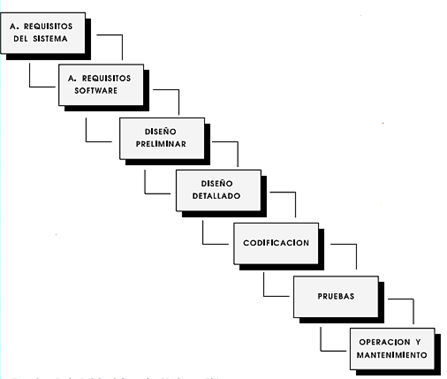
\includegraphics[width=0.8\textwidth]{fig/cascada.png}
\end{center}
\caption{Etapas del Modelo en Cascada}
\label{fig:cascada}
\hrule
\end{figure}

\paragraph{Ventajas}
Este modelo es ideal, generalmente, para proyectos grandes de carácter
estable (en especial aquellos que no tengan posibilidad de cambio en
los requisitos), es decir, proyectos donde es posible predecir de
manera completa el área del problema a resolver y así los diseñadores
puedan definir un diseño correcto y completo antes de comenzar las
fases de implementación. Por otro lado, este modelo también puede ser
utilizado en proyectos de menor envergadura donde todos los requisitos
estén bien establecidos.
 
La organización de este modelo y su diferenciación en las fases hace
que su utilización sea sencilla ya que esta rigidez produce que cada
fase tenga unos pasos bien definidos y unos entregables específicos y
un proceso de revisión de la fase, por lo que cada fase se
realiza. procesa y completa de una vez.


\paragraph{Inconvenientes}

El mayor inconveniente es que en la vida real es difícil encontrar
proyectos de ingeniería del software donde exista dicha estabilidad y
mucho menos sigan un proceso secuencial, por lo que la utilización de
este modelo resultaría una elección equivocada que conlleva al fracaso
del proyecto.
 
Otro inconveniente es que todos los resultados o mejoras que se pueden
ir haciendo no son visibles de manera progresiva, solo pueden verse
cuando el producto está terminado, esto puede provocar una inseguridad
y desconfianza por parte del cliente que siempre gusta de ir viendo
avances en el producto y opinar sobre el camino que está tomando. Esto
afecta también en el momento de tener que añadir un requisito que no
fue tomado en cuenta al comienzo del proyecto, y que surgió,
seguramente, en la etapa de la codificación. Este hecho sucede
bastante a menudo y en este modelo te obliga a volver a la etapa de
requisitos y repetir tareas ya finalizadas.

\section{Modelo de Prototipos}
\label{sec:prototipos}
El modelo basado en prototipos no determina una serie de etapas sino
que define un comportamiento en cada etapa. La construcción de
prototipos ha de comenzar desde la primera etapa del ciclo de vida del
software, es decir desde la recolección y especificación de requisitos
primera. Para llevar a cabo este modelo, es necesario que el
desarrollador y el cliente se encuentren y definan cuáles serán los
objetivos globales del software a desarrollar, así como identificar
los requisitos conocidos. A partir de esta información se debe
realizar un diseño rápido que se centre en representar esos aspectos
que serán más visible para el usuario o cliente, este diseño se
concreta en la elaboración de un prototipo. El prototipo será evaluado
y se irá refinando junto con los requisitos del software. Los avances
en las etapas permiten al cliente ver como va el proyecto y al
desarrollador comprender qué es lo que el cliente quiere que haga.

\begin{figure}[h]
\hrule\smallskip
\begin{center}
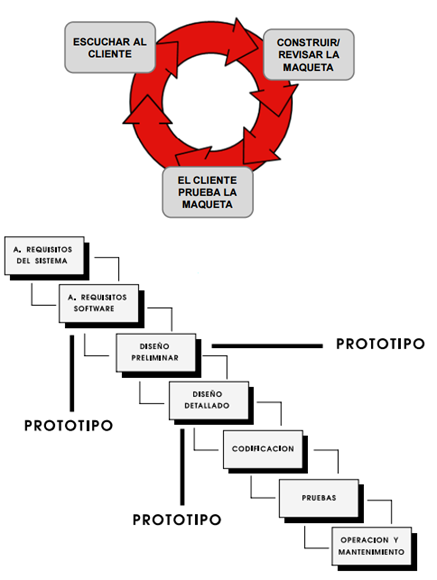
\includegraphics[width=0.5\textwidth]{fig/prototipo.png}
\end{center}
\caption{Ejemplo del Modelo de prototipos y Ciclo de trabajo.}
\label{fig:prototipos}
\hrule
\end{figure}

Se puede hacer un prototipado de diferentes maneras:
\begin{itemize}
\item Prototipado rápido:
  \begin{itemize}
  \item No modifica el ciclo de vida.
  \item Baja calidad y robustez.
  \item Evita producir cosas no solicitadas por el cliente.
  \item Reduce costes.
  \end{itemize}
\item Prototipado evolutivo:
  \begin{itemize}
  \item Funcionalidad progresiva.
  \item Construir software para que pueda ser modificado fácilmente.
  \item No se conocen niveles apropiados de calidad y documentación.
  \end{itemize}
\item Prototipado operacional:
  \begin{itemize}
  \item Mezcla rápido y evolutivo.
  \item Se basa en la siguiente imagen.
  \end{itemize}
\end{itemize}


\paragraph{Ventajas}

Este modelo de proceso tiene la gran ventaja de poder observar desde
el comienzo del ciclo de vida del software versiones posibles del
producto (los prototipos). Con ello, tal y como se ha comentado
anteriormente, el cliente puede conseguir definir mejor qué
necesidades reales tiene y cuáles son los requisitos del
producto. Esta realimentación continua del cliente nos lleva a evitar
malas sorpresas al final del proceso.

Cada prototipo puede sustituir a los documentos que indican la
situación del proyecto, aportando una realidad visual del estado del
proyecto. Además deja entrever el buen funcionamiento que tendrá el
producto final.

\paragraph{Inconvenientes}
El mayor inconveniente de este modelo es la propia realización de
prototipos que en muchos casos son productos que requieren una
inversión y que acabarán en la basura, aunque se haya aprendido
gracias a él. Si no se controla y elige bien el tipo de prototipo a
realizar puede conllevar un aumento de los costes del desarrollo del
producto.

Además, tener versiones semi-funcionales y mostrarlas al cliente
pueden llevar a una falsa ilusión del buen avance del proyecto, si no
comprende la utilidad y finalidad de los prototipos. Por último, el
desarrollador puede comprometer la calidad y el mantenimiento del
software dado que para un prototipo se puede ``cablear'' una solución
temporal que después conlleve cambios en los diseños.

\section{Modelo Incremental}
\label{sec:incremental}

Este modelo de proceso combina los dos anteriores, de modo que obtiene
la filosofía interactiva del modelo basado en prototipos y la
fiabilidad del modelo en cascada. Este modelo va incrementando la
funcionalidad del software, de modo que se aplica el modelo en cascada
con un conjunto de requisitos limitados a una o dos funcionalidades y
al terminar el producto es un prototipo, al realizar este proceso
añadiendo funcionalidades vas obteniendo diferentes prototipos hasta
que consigues el producto final.

Algunas de las principales características del modelo incremental son
las siguientes:
\begin{itemize}
\item Soluciona el problema del modelo en cascada eliminando la
  secuenciación lineal.
\item El producto final es el resultado de ir añadiendo componentes
  funcionales en forma de incrementos.
\item El software es analizado en partes de modo que no se ve como un
  producto a entregar a una fecha fija, sino como un producto
  resultado de trabajos incrementales.
\item Al ir añadiendo funcionalidades se puede adaptar a entornos
  donde hay incertidumbre en los requisitos, de modo que se van
  desarrollando funcionalidades según van apareciendo necesidades.
\end{itemize}

  

\begin{figure}[h]
\hrule\smallskip
\begin{center}
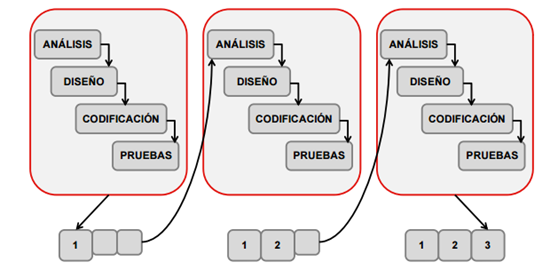
\includegraphics[width=0.8\textwidth]{fig/iterativo.png}
\end{center}
\caption{Modelo Incremental de tres fases.}
\label{fig:iterativo}
\hrule
\end{figure}

\paragraph{Ventajas} Las ventajas más importantes de este modelo corresponden con sus principales características, además aporta otras ventajas como:
\begin{itemize}
\item Reduce el coste en los cambios de alcance o requisitos del
  software.
\item Se simplifican las tareas de testing y depuración al solo tener
  que analizar una iteración pequeña cada vez.
\item Los riesgos referentes al desarrollo son más gestionables debido
  a que una iteración no contiene la totalidad del desarrollo, que
  suceda un riesgo afectaría al desarrollo de una funcionalidad y no
  al producto completo.
\item Al igual que el modelo basado en prototipos, cada iteración
  corresponde a un hito en el programa del proyecto que es fácilmente
  gestionable.
\end{itemize}


\paragraph{Inconvenientes}
Este modelo presenta varios inconvenientes, uno de ellos es la
necesidad de experiencia en el equipo para definir incrementos de modo
que no sean excesivamente pequeños ni demasiado grandes para poder
distribuir el trabajo de forma proporcionada y no realizar iteraciones
con todo su coste para un incremento insignificante. Otros
inconvenientes que aparecen al utilizar este modelo son:
\begin{itemize}
\item Cada iteración es secuencial y no es posible superponerlas entre
  sí.
\item Al no definir todos los requisitos completos al inicio pueden
  surgir incompatibilidades entre los mismos. Además, pueden dar
  problemas en la arquitectura del software, dado que en las primeras
  iteraciones se ha podido no preparar bien para integrar alguna
  funcionalidad de iteraciones posteriores.
\end{itemize}


\section{Modelo en Espiral}
\label{sec:espiral}

Barry Boehm en 1985 desarrolló el modelo en espiral, publicado en 1988
en el artículo ``A Spiral Model of Software Development and
Enhancement'', que ha sido y es utilizado de forma muy
generalizada en todo el ámbito de la ingeniería del software. El
nombre del modelo proviene de la forma en que se propone colocar las
actividades y etapas del desarrollo del software. Esta forma es una
espiral partiendo del centro, y cada vuelta corresponde a un ciclo
completo en que las actividades de ese ciclo se fijan en función de
los análisis y resultados del ciclo anterior.\\

 
Al igual que el modelo iterativo, este modelo parte de ideas básicas
del modelo basado en prototipos y el modelo en cascada. Este modelo
resulta idóneo para proyectos de larga duración, que sean caros y
complejos en su elaboración.\\

Cada ciclo de la espiral debe pasar por al menos cuatro etapas. La
primera de ellas es determinar y fijar objetivos, esto incluye
determinar los entregables, y realizar la planificación. La segunda
etapa es la encargada de hacer un análisis de riesgos estudiando
alternativas para reducirlos y eliminarlos. Como tercera etapa se
contempla todo el proceso de desarrollo, verificación y validación del
software, es la etapa de propia de creación y programación. En la
cuarta y última etapa, se revisa todo el trabajo realizado, se evalúa
y se pre-planifican las siguientes fases, y en concreto el siguiente
ciclo. Podemos observar este proceso en la Figura~\ref{fig:espiral}
comenzando en el centro y siguiendo hacia afuera en el sentido de las
agujas del reloj.

\begin{figure}[h]
\hrule\smallskip
\begin{center}
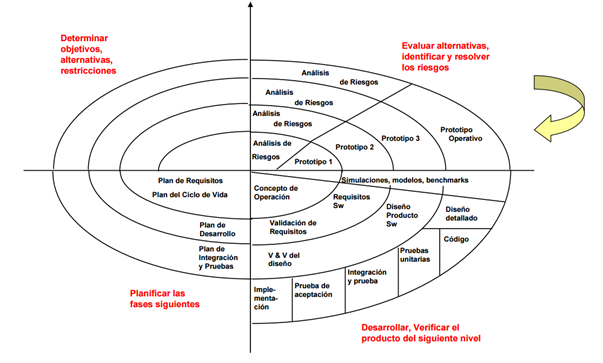
\includegraphics[width=0.7\textwidth]{fig/espiral.png}
\end{center}
\caption{Modelo en Espiral}
\label{fig:espiral}
\hrule
\end{figure}

\paragraph{Ventajas} Al realizarse el análisis de riesgos de una modo
claro y explícito se consigue reducir los riesgos del proyecto y
permite incorporar objetivos centrados en obtener calidad. Además
pueden añadirse ciclos donde se desarrolle el mantenimiento del
software. Añadir nuevos requisitos y mejoras puede hacerse sin romper
el modelo o volver a empezar, todo gracias a que el ciclo de vida no
es rígido.

\paragraph{Inconvenientes} Quizá su mayor problema es que utilizar
este modelo conlleva realizar mucho trabajo adicional, por la alta
exigencia que tiene en los análisis de riesgos. Esto conlleva a
necesitar experiencia y analistas expertos en esta tarea. Este modelo
es prácticamente incompatible con proyectos pequeños dado que no
necesitaría más que una vuelta.
